\section{Interfejs komunikacyjny}
    \tab Wiele nowoczesnych urządzeń wykorzystuje rozmaite standardy i interfejsy komunikacyjne do różnych celów.
    Tak samo powyższy projekt wykorzystuje kilka prostych standardów do komunikacji zarówno z użytkownikiem oraz peryferiami.

    \subsection{Standard UART i interfejs bluetooth}
        \tab Podstawowym sposobem komunikacji z użytkownikiem jest protokół UART, wraz z interfejsem Bluetooth.
        Standard komunikacji UART, jest to prosty dwukierunkowy asynchroniczny sposób do przesyłania danych między dwoma urządzeniami.\\
        Opis przykładowej ramki w standardzie UART:
            
        \begin{figure}[!ht]
            \centering
            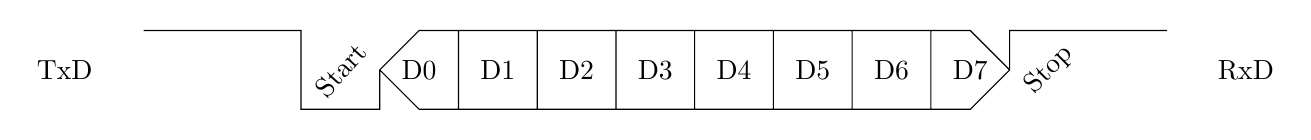
\begin{tikzpicture}
                \draw
                (-1, 0.5) node[]{TxD}
                (0, 1) -- (2, 1)
                    -- (2, 0)
                    -- (3, 0)
                    -- (3, 0.5) coordinate(start) ++(-0.5, 0) node[rotate = 48]{Start}

                (start) --++ (0.5, -0.5) -- ++ (7, 0) --++(0.5, 0.5) coordinate(stop)
                (start) --++ (0.5, 0.5) -- ++ (7, 0) --++(0.5, -0.5)

                (start) ++ (1, 0.5) -- ++ (0, -1) ++ (-0.5, 0.5) node[]{D0}
                (start) ++ (2, 0.5) -- ++ (0, -1) ++ (-0.5, 0.5) node[]{D1}
                (start) ++ (3, 0.5) -- ++ (0, -1) ++ (-0.5, 0.5) node[]{D2}
                (start) ++ (4, 0.5) -- ++ (0, -1) ++ (-0.5, 0.5) node[]{D3}
                (start) ++ (5, 0.5) -- ++ (0, -1) ++ (-0.5, 0.5) node[]{D4}
                (start) ++ (6, 0.5) -- ++ (0, -1) ++ (-0.5, 0.5) node[]{D5}
                (start) ++ (7, 0.5) -- ++ (0, -1) ++ (-0.5, 0.5) node[]{D6}
                (start) ++ (8, 0.5) ++ (0, -1) ++ (-0.5, 0.5) node[]{D7}
                % (start) ++ (8.5, 0) node[]{P}

                (stop) --++(0, 0.5) -- ++(2, 0) coordinate(end)
                (stop) ++ (0.5, 0) node[rotate = 45]{Stop}
                (end) ++ (1, -0.5) node[]{RxD}
                        
                ;
            \end{tikzpicture}
            \caption{Ramka danych w standardzie UART}
        \end{figure}
% 
        \noindent
        W tym projekcie komunikacja odbywa się z szybkością 9600baud'ów (Do zmiany prawie na 100\%).
        Dodatkowo, standard pozwala na przesyłanie dodatkowego bity parzystości ,,doklejanego" do końca wiadomości, jako sposób sprawdzania poprawności wysłanej wiadomości.

        Dalszą częścią kanału transmisyjnego jest przekaźnik bluetooth, który łączy się z komputerem na odpowiednim porcie szeregowym łatwym do oczytania dla programu napisanego na komputerze.
    
    \subsection{Interfejs Two Wire (I²C)}
        \tab Ostatnim interfejsem, wykorzystywanym przez „Azora” jest interfejs I$^2$C -- czyli dwukierunkowa szeregowa magistrala OC z układ Master-Slave.
        Standard ten służy do połączenie urządzeń peryferyjnych z kontrolerem.
        Komunikacja odbywa się w 8bitowych ramkach, z tym że pierwsza ramka zawsze definiuje adres urządzenia docelowego oraz określa kierunek transmisji „do” lub „z”~urządzenia.

        \begin{figure}[!ht]
            \centering
            \begin{circuitikz}
                \draw
                    (0, 0) node[draw, rectangle, minimum width = 2cm, minimum height = 2cm](Master){Master}
                    (0, -3.5) node[draw, rectangle, minimum width = 2cm, minimum height = 2cm](Slave1){Slave 1}
                    (2.5, -3.5) node[draw, rectangle, minimum width = 2cm, minimum height = 2cm](Slave2){Slave 2}
                    (5, -3.5) node[draw, rectangle, minimum width = 2cm, minimum height = 2cm](Slave3){Slave 2}

                    (0.25, -1.5) coordinate(clk) -- (5.5, -1.5) ++ (-1, 0) node[above]{$CLK$}
                    (0.25, -1.5) to[short, *-] ++ (0, 0.5) 
                        
                    (-0.25, -2.25) coordinate(sda) -- (5, -2.25) ++ (-1, 0) node[above]{$SDA$}
                    (-0.25, -2.25) to[short, *-] ++ (0, 1.25) 

                    ( 0.25, -1.5) -- ++ (0, -1)
                    (-0.25, -2.25) -- ++ (0, -0.25)
                        
                    (2.75, -1.5) to[short, *-] ++ (0, -1)
                    (2.25, -2.25) to[short, *-] ++ (0, -0.25)

                    (5.5, -1.5) to[short, -] ++ (0, -1)
                    (5.0, -2.25) to[short, -] ++ (0, -0.25)

                    (clk) -- ++ (-2.5, 0) to[R] ++ (0, 2) node[vcc]{+5V}
                    (sda) -- ++ (-3.0, 0) -- ++ (0, 0.75) to[R] ++(0, 2) node[vcc]{+5V}
                ;
            \end{circuitikz}
            \caption{Schemat blokowy magistrali I$^2$C}
        \end{figure}

\newpage
    \subsection{Interfejs SPI}
        % źródło: http://extronic.pl/content/60-kurs-xmega-interfejs-spi
        \tab Procesor bez programu, jest bezużytecznym kawałkiem krzemu dlatego niezwykle istotnym jest zaprogramowanie układu.
        Podstawową metodą programowania układów z rodziny ATmega jest interfejs SPI. 

        \begin{figure}[!ht]
            \centering
            \begin{tikzpicture}
                \draw
                    (0, 0) -- (0, 8) -- (1, 8) -- (1, 0) -- (0, 0)
                    (0, 1) -- (1, 1) ++ (-0.5, -0.5) node[](MD0){D0}
                    (0, 2) -- (1, 2) ++ (-0.5, -0.5) node[]{D1}
                    (0, 3) -- (1, 3) ++ (-0.5, -0.5) node[]{D2}
                    (0, 4) -- (1, 4) ++ (-0.5, -0.5) node[]{D3}
                    (0, 5) -- (1, 5) ++ (-0.5, -0.5) node[]{D4}
                    (0, 6) -- (1, 6) ++ (-0.5, -0.5) node[]{D5}
                    (0, 7) -- (1, 7) ++ (-0.5, -0.5) node[]{D6}
                                        ++       (0, 1) node[](MD7){D7}
                    (2, -1.5) -- (2, 9)

                    (8, 0) -- (8, 8) -- (9, 8) -- (9, 0) -- (8, 0)
                    (8, 1) -- (9, 1) ++ (-0.5, -0.5) node[](SD7){D7}
                    (8, 2) -- (9, 2) ++ (-0.5, -0.5) node[]{D6}
                    (8, 3) -- (9, 3) ++ (-0.5, -0.5) node[]{D5}
                    (8, 4) -- (9, 4) ++ (-0.5, -0.5) node[]{D4}
                    (8, 5) -- (9, 5) ++ (-0.5, -0.5) node[]{D3}
                    (8, 6) -- (9, 6) ++ (-0.5, -0.5) node[]{D2}
                    (8, 7) -- (9, 7) ++ (-0.5, -0.5) node[]{D1}
                                        ++       (0, 1) node[](SD0){D0}
                    (7, -1.5) -- (7, 9)

                        
                    (-2.75, -1.25) rectangle ++ (2, 1)
                    (-1.75, -0.75) node[](clk){Clk} 
                    (clk) ++ (1, 0) coordinate(clk)
                    (clk) -- ++ (0.5, 0)
                        to[short, *-] ++ (0, 1.25) coordinate(MD)
                        to[short, *-] ++ (0.25, 0)
                    (MD) -- ++ (0, 1) coordinate(MD)
                        to[short, *-] ++ (0.25, 0)
                    (MD) -- ++ (0, 1) coordinate(MD)
                        to[short, *-] ++ (0.25, 0)
                    (MD) -- ++ (0, 1) coordinate(MD)
                        to[short, *-] ++ (0.25, 0)
                    (MD) -- ++ (0, 1) coordinate(MD)
                        to[short, *-] ++ (0.25, 0)
                    (MD) -- ++ (0, 1) coordinate(MD)
                        to[short, *-] ++ (0.25, 0)
                    (MD) -- ++ (0, 1) coordinate(MD)
                        to[short, *-] ++ (0.25, 0)
                    (MD) -- ++ (0, 1) coordinate(MD)
                        to[short] ++ (0.25, 0)

                    (clk) -- ++ (10, 0) coordinate(SD)
                    (SD) to[short, -] ++ (0, 1.25) coordinate(SD)
                        -- ++(-0.25, 0)
                    (SD) to[short, *-] ++ (0, 1) coordinate(SD)
                        -- ++(-0.25, 0)
                    (SD) to[short, *-] ++ (0, 1) coordinate(SD)
                        -- ++(-0.25, 0)
                    (SD) to[short, *-] ++ (0, 1) coordinate(SD)
                        -- ++(-0.25, 0)
                    (SD) to[short, *-] ++ (0, 1) coordinate(SD)
                        -- ++(-0.25, 0)
                    (SD) to[short, *-] ++ (0, 1) coordinate(SD)
                        -- ++(-0.25, 0)
                    (SD) to[short, *-] ++ (0, 1) coordinate(SD)
                        -- ++(-0.25, 0)
                    (SD) to[short, *-] ++ (0, 1) coordinate(SD)
                        -- ++(-0.25, 0)

                    (MD7) ++ (0.5, 0) coordinate (MD7)
                    (SD0) ++ (-0.5,0) coordinate (SD0)
                    (MD0) ++ (0.5, 0) coordinate (MD0)
                    (SD7) ++ (-0.5,0) coordinate (SD7)

                    (MD7) -- (SD0)
                    (MD0) -- (SD7)
                        
                    (MD7) ++ (4, 0) -- ++ (-0.2, 0.2)
                    (MD7) ++ (4, 0) -- ++ (-0.2, -0.2)
                    (MD7) ++ (2.2, 0) node[above]{MOSI}
                    % (SD7) ++ (-2.2, 0) node[above]{MISO}

                    (MD0) ++ (4, 0) -- ++ (0.2, 0.2)
                    (MD0) ++ (4, 0) -- ++ (0.2, -0.2)
                    (MD0) ++ (2.2, 0) node[above]{MISO}
                    % (SD0) ++ (-2.2, 0) node[above]{MOSI}

                    (MD7) ++ (0, 1) node[]{MASTER}
                    (SD0) ++ (0, 1) node[]{SLAVE}
                ;

            \end{tikzpicture}
            \caption{Schemat interfejsu SPI}
        \end{figure}
        \noindent
        W przeciwieństwie do poprzednio omawianego interfejsu,
        SPI jest interfejsem typu Master-Slave -- wyróżniamy układ sterujący (Master),
        którego zadaniem jest wyznaczenie taktowania zegara 
        oraz zarządzanie magistralą układami układami podrzędnymi (Slave), poprzez wystawienie stanu aktywnego na pinie \textit{,,CS"}.

        % Dodatkowo, urządzenia slave posiadają specjalne wejście ,,CS", których aktywacja zezwala na komunikację za pomocą protokołu SPI.
        

    \newpage
            

        
            